\documentclass[conference]{IEEEtran}
\IEEEoverridecommandlockouts
% The preceding line is only needed to identify funding in the first footnote. If that is unneeded, please comment it out.
\usepackage{cite}
\usepackage{amsmath, amsfonts, amsthm, amssymb}  % Some math symbols
\usepackage{enumerate}
\usepackage{enumitem}
\usepackage{hyperref}
\usepackage{algorithmic}
\usepackage{graphicx}
\usepackage{textcomp}
\usepackage{xcolor}
\usepackage{natbib}
\usepackage{wrapfig}
\usepackage{changepage}
\usepackage{subfig}
\usepackage{float}
\usepackage{setspace}
\usepackage{hhline}
\usepackage{makecell}
\usepackage[all]{xy}
\usepackage{fancyvrb}
\usepackage[T1]{fontenc}
\usepackage{listings}
\usepackage{fancyhdr}
\usepackage{mathtools}
\usepackage{capt-of}
\usepackage{gensymb}
\usepackage{epstopdf}
\usepackage{booktabs}
\usepackage{xcolor}
\usepackage{centernot}

\DeclarePairedDelimiter{\ceil}{\lceil}{\rceil}
\DeclarePairedDelimiter{\floor}{\lfloor}{\rfloor}
\DeclarePairedDelimiter{\card}{\vert}{\vert}

\usepackage[style=ieee]{biblatex}
\DeclareLanguageMapping{english}{english-apa}
\addbibresource{references.bib}

\def\BibTeX{{\rm B\kern-.05em{\sc i\kern-.025em b}\kern-.08em
    T\kern-.1667em\lower.7ex\hbox{E}\kern-.125emX}}
    
\pagestyle{head}

%%%%%%% ONE COLUMN %%%%%%% 
\onecolumn

%%%%%%% BEGIN DOCUMENT %%%%%%% 
\begin{document}

\title{\LARGE Design of a IEEE 802.11 Based WiFi Mesh Network \\ for Low Power IoT Devices\\
{\Large A Capstone Proposal}
}

\author{
    \IEEEauthorblockN{Barkin Simsek}
    \IEEEauthorblockA{
        Computer Engineering
        \\
        \textit{bs3528@nyu.edu}
    }
    
    \and
    
    \IEEEauthorblockN{Nishant Aswani}
    \IEEEauthorblockA{
        Computer Engineering
        \\
        \textit{nsa325@nyu.edu}
    }
}


\maketitle

%\begin{abstract}
%This document is a model and instructions for \LaTeX.
%This and the IEEEtran.cls file define the components of your paper [title, text, heads, etc.]. *CRITICAL: Do Not Use Symbols, Special Characters, Footnotes, 
%or Math in Paper Title or Abstract.
%\end{abstract}

\noindent \textbf{Faculty Advisors:}
Our faculty advisors are Matthew Karau (mbk7@nyu.edu) and Saif E. Jabari (sej7@nyu.edu)

% \begin{IEEEkeywords}

% \end{IEEEkeywords}

\section{Statement of Project Summary}
In this project, we will develop a low cost and highly scalable IEEE 802.11 based WiFi mesh network for low power Internet of Things (IoT) devices. Network simulations will be carried out for testing the preliminary designs and optimizing the mesh network design. Later, the designed mesh network will be implemented as a software library for ESP8266, which is one of the most popular embedded microcontroller units available for building IoT devices. Criteria like speed, ease of use, cost, stability, compatibility with legacy devices, packet loss percentage, and network throughput will be considered while designing the mesh network.\\

We will use the implemented software library as a proof of concept for our mesh network design. It will be also useful for benchmarking our design to compare with potential competitors and further optimizing our mesh network design. After finishing the capstone, the designed and implemented IEEE 802.11 based WiFi mesh network software library will be publicly available to the open source community at large for further testing and collaboration.

\section{Background and Review of Literature}
Networks are an integral part of describing natural and artificial systems, such as networks of neurons in our brain or computer networks. How elements of a network are connected plays a crucial importance in the network's efficiency, health, and resilience against failures. For example, in the 2003 North American Blackout, a local failure in Ohio caused the entire North American power grid network to go down, leaving millions of people in the dark \cite[]{blackout}. Experts say that this could have prevented if the power grid network was developed with a better structure in mind. Similarly, computer networks are prone to such cascading failures as well but are often prevented due to their distributed structure and built-in redundancies. The spread of a cascading failure in a network is depicted in Figure \ref{fig:failure}. \\

\begingroup
    \centering
    \medskip
    %width=\columnwidth
    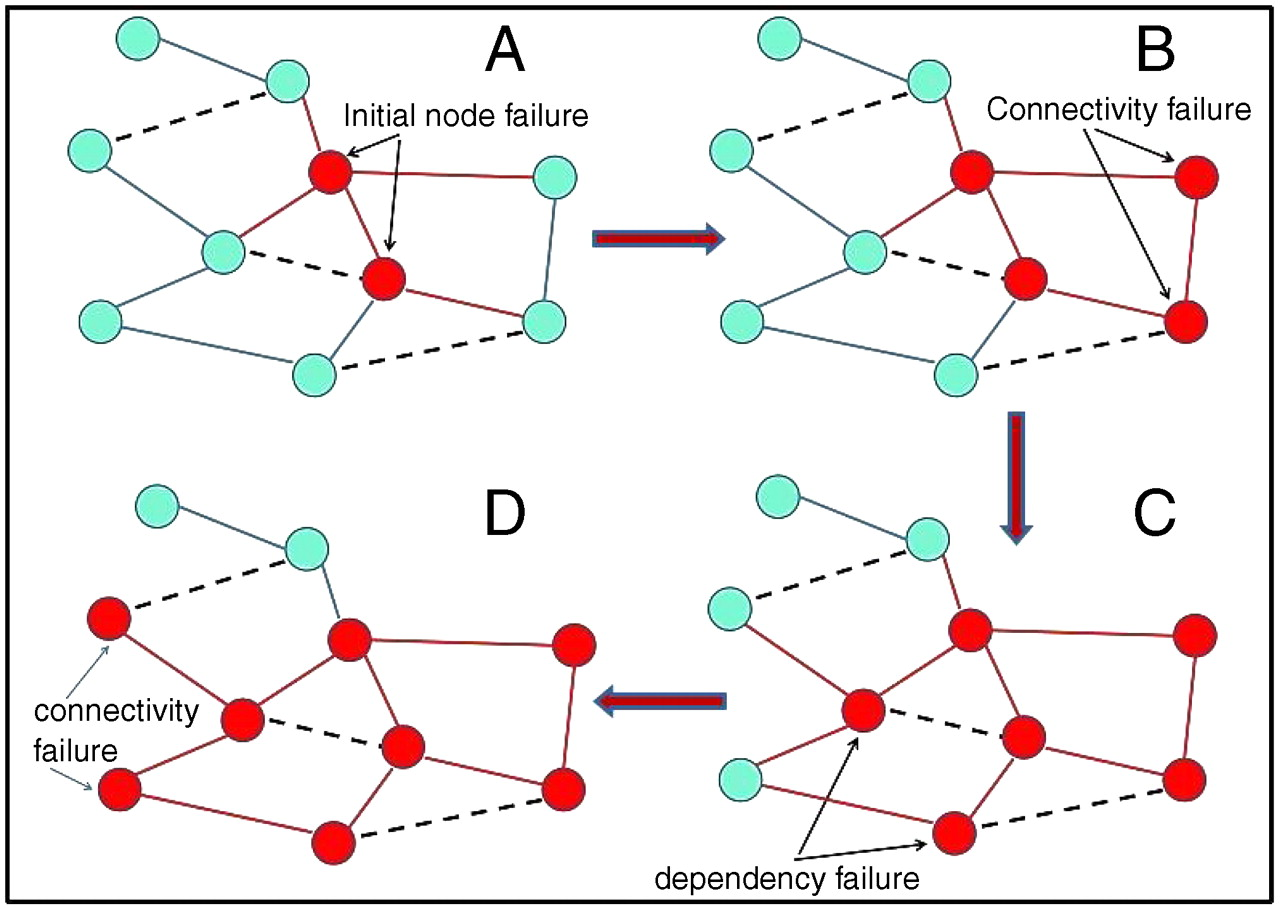
\includegraphics[width=0.4\columnwidth]{images/failure.jpg}
    \captionof{figure}{Cascading failures in networks \cite[]{Parshani_Buldyrev_Havlin_2011}}
    \label{fig:failure}
    \medskip
\endgroup

\noindent As a result, analysis, research, and modeling of new decentralized and mesh network architectures becomes imperative. In addition to these, the number of IoT devices are rapidly increasing due to their increasing popularity. Thus, new network architectures like mesh networking are required to reduce the burden on routers used in traditional networking systems.\\

Previously, mesh networks have been implemented in several wireless protocols such as LoRa \cite{Ochoa_Guizar_Maman_Duda_2017}\cite{Lee_Ke_2018}, Bluetooth  \cite{Leonardi_Patti_Lo_Bello_2018}, and ZigBee \cite{Rodriguez_Ortiz_Uriarte_Yi_Jia_Yoshii_Ross_Beckman_2011}. Mesh networking has been mainly implemented for PC grade hardware or for running on Linux operating systems \cite{Riggio_Miorandi_Chlamtac_Scalabrino_Gregori_Granelli_Fang_2008}\cite{Riggio_Gomez_Rasheed_Gerola_Miorandi_2009}. All of these solutions require purchasing expensive PC grade hardware or new radio antennas. As of now, there is no software library that enables mesh networking on the mainstream IEEE 802.11 based WiFi radios used on cheap and low power IoT devices.

\begingroup
    \centering
    \medskip
    %width=\columnwidth
    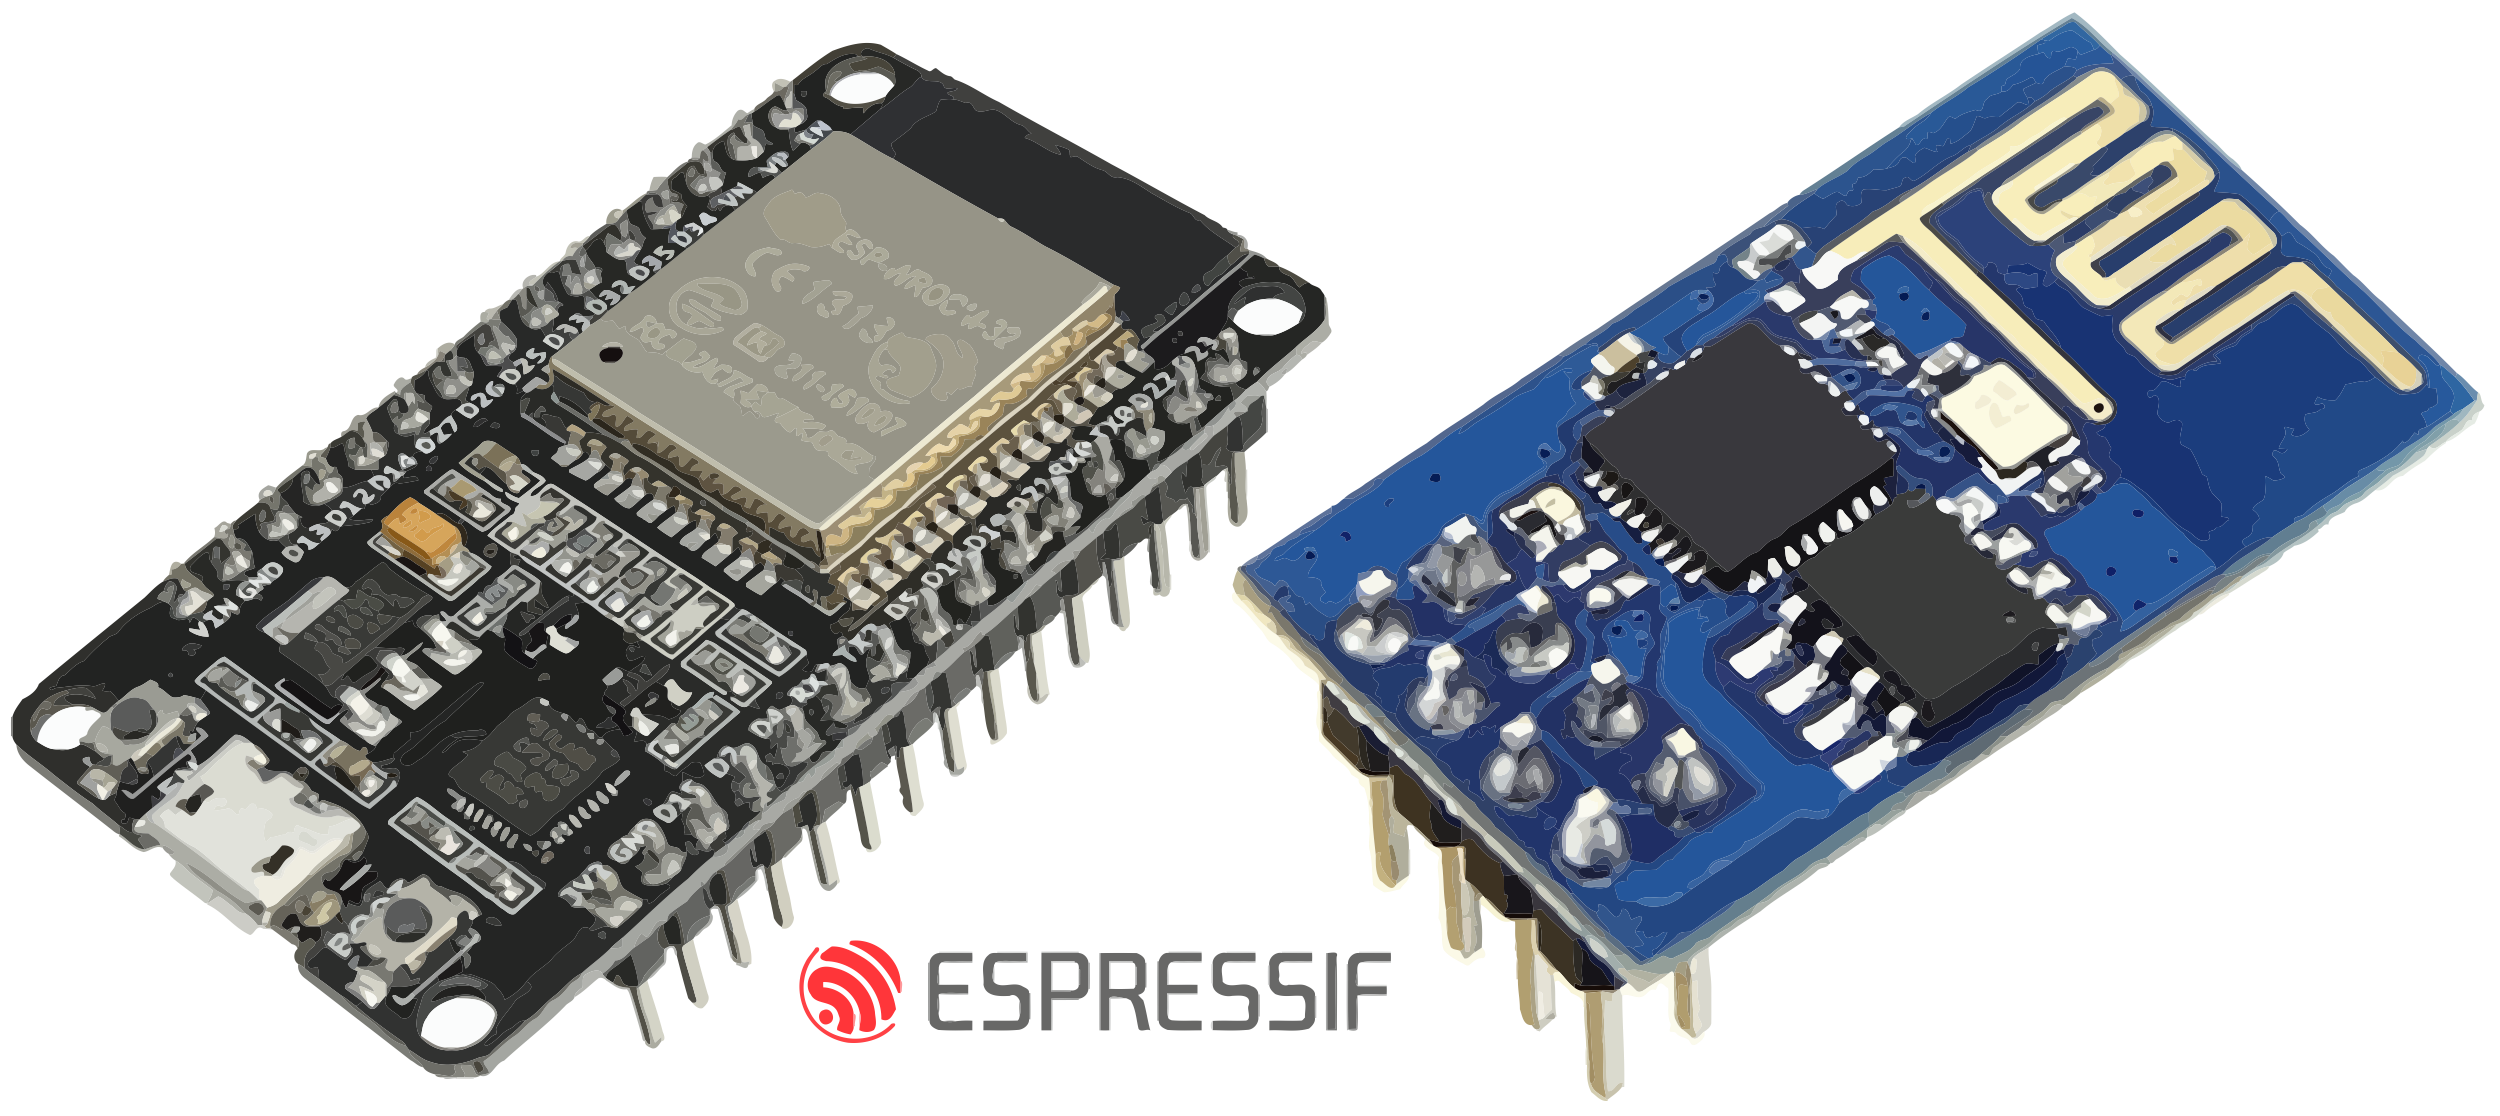
\includegraphics[width=0.4\columnwidth]{proposal/images/esp.png}
    \captionof{figure}{Some of the low power esp8266 based boards used in IoT devices \cite[]{esp}}
    \label{fig:failure}
    \medskip
\endgroup

Therefore, we have noticed a potential gap between available mesh networking solutions for IoT devices and practical needs. We realize that in order to take full advantage of mesh networking capabilities, engineers have to introduce new hardware into their systems. We propose a solution that creates an efficient mesh networking architecture for currently deployed devices without any major hardware upgrades to deployed systems.\\

\noindent \textit{Suggested readings for further information:}
\begin{itemize}
    \item Karimi, Kaivan, and Gary Atkinson. What the Internet of Things (IoT) Needs to Become a Reality. p. 16.
    \item Biswas, Sanjit, and Robert Morris. ExOR: Opportunistic Multi-Hop Routing for Wireless Networks. p. 11.
    \item Aguayo, Daniel, et al. Link-Level Measurements from an 802.11b Mesh Network. p. 11.
    \item \href{https://www.open-mesh.org/projects/batman-adv/wiki/Quick-start-guide}{Better Approach To Mobile Adhoc Networking (B.A.T.M.A.N.)}
    \item \href{https://openthread.io/guides/thread-primer}{Thread Network Protocol}
    \item Texas Instruments, Reiter, Gil. A Primer to Wi-Fi Provisioning for IoT Applications. 2019, p. 7.
    \item Texas Instruments, Wireless Connectivity for the Internet of Things, One Size Does Not Fit All. 2014, p. 13.
    \item Raniwala, A., and Tzi-cker Chiueh. “Architecture and Algorithms for an IEEE 802.11-Based Multi-Channel Wireless Mesh Network.” Proceedings IEEE 24th Annual Joint Conference of the IEEE Computer and Communications Societies., vol. 3, 2005, pp. 2223–34 vol. 3. IEEE Xplore, doi:10/bw2t5q.
    \item Bansal, Divya, and Sanjeev Sofat. “Deployment and Evaluation of IEEE 802.11 Based Wireless Mesh Networks in Campus Environment.” Proceedings of the 4th ACM Workshop on Networked Systems for Developing Regions, ACM, 2010, pp. 15:1–15:2. ACM Digital Library, doi:10.1145/1836001.1836016.
    \itme Ferrari, Federico, et al. “Efficient Network Flooding and Time Synchronization with Glossy.” Proceedings of the 10th ACM/IEEE International Conference on Information Processing in Sensor Networks, 2011, pp. 73–84.
    \item Song, Heecheol, et al. “IEEE 802.11-Based Wireless Mesh Network Testbed.” 2007 16th IST Mobile and Wireless Communications Summit, 2007, pp. 1–5. IEEE Xplore, doi:10/cvqwj2.
    \item Gupta, P., and P. R. Kumar. “The Capacity of Wireless Networks.” IEEE Transactions on Information Theory, vol. 46, no. 2, Mar. 2000, pp. 388–404. DOI.org (Crossref), doi:10/bqf9fp.
    \item Cilfone, Antonio, et al. “Wireless Mesh Networking: An IoT-Oriented Perspective Survey on Relevant Technologies.” Future Internet, vol. 11, no. 4, Apr. 2019, p. 99. DOI.org (Crossref), doi:10/ggdrkv.
\end{itemize}




\section{Resources Information}
\begin{itemize}
    \item A computer with internet connection 
        \begin{itemize}
            \item Preferably Ubuntu as the operating system
        \end{itemize}
    \item esp8266 development boards
        \begin{itemize}
            \item Available in the Engineering Design Studio
            \item At least 10 boards are required to demonstrate the proposed mesh network design
            \item \href{https://www.adafruit.com/product/2471}{https://www.adafruit.com/product/2471}
        \end{itemize}
    \item NS-3, Cloonix, CORE, OMNeT++ network simulation software
        \begin{itemize}
            \item All of these simulation software are open-source and freely available
        \end{itemize}
\end{itemize}
\section{Publication/Patents}
\noindent Results of the capstone project are planned to be submitted to related journals. Additionally, created open-source code would leave a legacy behind that anyone who needs to implement a network structure mentioned above can freely use the generated code. This legacy would also contribute to recognition of NYU Abu Dhabi in the open-source community at large.

\section{Project Timeline}
\noindent The details of the projected capstone project timeline is provided in the Table \ref{fig:timeline}. Proposed dates might be revised based on the progress on the corresponding stage of the project. The ultimate aim is coming back to school in our Senior year with a ready to implement and mature capstone idea.

\begingroup
    \bigskip
    \centering
    \def\arraystretch{1.2}
        \begin{tabular}{lll}
            \toprule
            \textbf{Time} & \textbf{Task Description} & \textbf{Deliverable} \\
            \midrule
            Spring 1 2020 & Background and literature review & Literature Summary\\ 
            \midrule
            Spring 2 2020 & Investigating the feasibility of the proposed project & Modified Capstone Proposal\\ 
            \midrule
            Summer 2020 &   Further literature review  & Literature Summary\\ 
            \midrule
            Fall 1 2020 & Investigating the feasibility of the modified proposal  & Progress Report\\ 
            \midrule
            Fall 2 2020 & Evaluating the final design with the help of professionals in mesh networking  & Finalized Capstone Proposal\\ 
            \midrule
            J-term 2021 & Continue to work on capstone & \\ 
            \midrule
            Spring 1 2021 & Implementing the proposed and refined design & Intermediate Report\\ 
            \midrule
            Spring 2 2021 & Testing, validating, and evaluation the implemented solution  & Capstone Report\\ 
            \bottomrule
        \end{tabular}
    \captionof{table}{projected capstone project timeline}
    \label{fig:timeline}
    \medskip
\endgroup



\printbibliography

\end{document}
